\documentclass[aspectratio=169]{beamer}

\usetheme{Madrid}
\usecolortheme{whale}
\setbeamertemplate{navigation symbols}{}

\usepackage[utf8]{inputenc}
\usepackage[T1]{fontenc}
\usepackage{lmodern}
\usepackage{booktabs}
\usepackage{tabularx}
\usepackage{array}
\usepackage{hyperref}
\usepackage{xcolor}
\usepackage{graphicx}

\hypersetup{
  colorlinks=true,
  linkcolor=blue!50!black,
  urlcolor=blue!50!black
}

\newcommand{\code}[1]{\texttt{\detokenize{#1}}}
\newcommand{\repo}{\texorpdfstring{\code{section_GNN}}{section_GNN}}
\newcolumntype{Y}{>{\raggedright\arraybackslash}X}

\title[Implementation Documentation for \repo]{Implementation-Level Documentation\\for \repo}
\author{Generated from the inspected repository state}
\date{March 31, 2026}

\begin{document}

\begin{frame}
  \titlepage
\end{frame}

\begin{frame}{Contents}
  \tableofcontents
\end{frame}

\section{Scope}

\begin{frame}{What This Deck Documents}
This slide deck documents the code that currently exists in \repo{}, not a generic legal GNN design.

\vspace{0.4cm}

\begin{itemize}
  \item Raw JSON to cleaned case preprocessing
  \item Exact graph ontology: all node types and edge types
  \item PyG feature construction and graph bundle contents
  \item Hetero GNN architecture and exact \code{forward()} behavior
  \item Label mapping, splitting, training, evaluation, and outputs
  \item Config variants, visualization tooling, limitations, and extension points
\end{itemize}
\end{frame}

\section{Codebase Map}

\begin{frame}{Repository Layout}
\small
\begin{tabularx}{\textwidth}{>{\raggedright\arraybackslash}p{0.23\textwidth}Y}
\toprule
Path Group & What Lives There \\
\midrule
\code{configs/} & Experiment YAMLs controlling paths, graph topology, labels, splits, model, training, and ablations. \\
\code{envs/} & Micromamba/conda environment definition. \\
\code{scripts/} & CLI entry points for preprocessing, graph build, training, ablation, and visualization export. \\
\code{src/preprocessing/} & Leakage masking, annotation filtering, normalization, and \code{CleanedCase} construction. \\
\code{src/graph/} & Schema dataclasses, local case graph builder, global merge, and PyG conversion. \\
\code{src/models/} & \code{HeteroLegalOutcomeGNN} and \code{MLPHead}. \\
\code{src/training/} & Label prep, split assignment, training loop, metrics, and plots. \\
\code{src/utils/} & I/O, logging, seeding, embedding cache, and pipeline orchestration. \\
\code{src/visualization/} & Static explanatory figure generation. \\
\code{visualiser/} & Browser-based D3 visualizer plus exported graph data. \\
\code{data/} and \code{outputs/} & Intermediate artifacts and run outputs, organized by experiment name. \\
\bottomrule
\end{tabularx}
\end{frame}

\begin{frame}{Primary Entry Points}
\small
\begin{tabularx}{\textwidth}{>{\raggedright\arraybackslash}p{0.34\textwidth}Y}
\toprule
Script & Runtime Role \\
\midrule
\code{scripts/preprocess_cases.py} & Read raw JSON files, build leakage-safe \code{CleanedCase} objects, and write cleaned cases, normalized entities, audits, and \code{preprocess_summary.json}. \\
\code{scripts/build_graph.py} & Load cleaned cases, build the global heterogeneous graph bundle, save \code{.pt} bundle and graph metadata. \\
\code{scripts/train_gnn.py} & Load graph cache, train once or across repeated seeds, save best run outputs. \\
\code{scripts/run_ablation.py} & Merge ablation overrides into a base config, rebuild the graph, train, and summarize variant results. \\
\code{scripts/visualize_graph.py} & Static graph-schema and message-passing figures. \\
\code{scripts/generate_final_visualisations.py} & Final explanatory PNGs about stored node features, edges, layers, and training. \\
\code{scripts/export_visualiser_catalog.py} & Browser fallback catalog export. \\
\code{scripts/export_training_graph_visualiser.py} & Exact training-graph export for the browser visualizer. \\
\bottomrule
\end{tabularx}
\end{frame}

\section{Pipeline}

\begin{frame}{End-to-End Pipeline}
\small
\begin{enumerate}
  \item Load raw case JSONs.
  \item Drop or mask leakage-bearing text and suspicious annotations.
  \item Normalize entities and derive side-specific lawyer and argument buckets.
  \item Serialize one \code{CleanedCase} JSON per case.
  \item Map labels to task classes and optionally drop procedural cases.
  \item Build one local case-star graph per retained case.
  \item Merge shareable nodes across cases into one hetero graph.
  \item Encode every node text into dense embeddings and append scalar features.
  \item Build \code{HeteroData} with labels and split masks on case nodes.
  \item Train the GNN on \code{case} nodes only, evaluate, and save artifacts.
\end{enumerate}
\end{frame}

\begin{frame}{Cross-Repository Pipeline Figure}
  \centering
  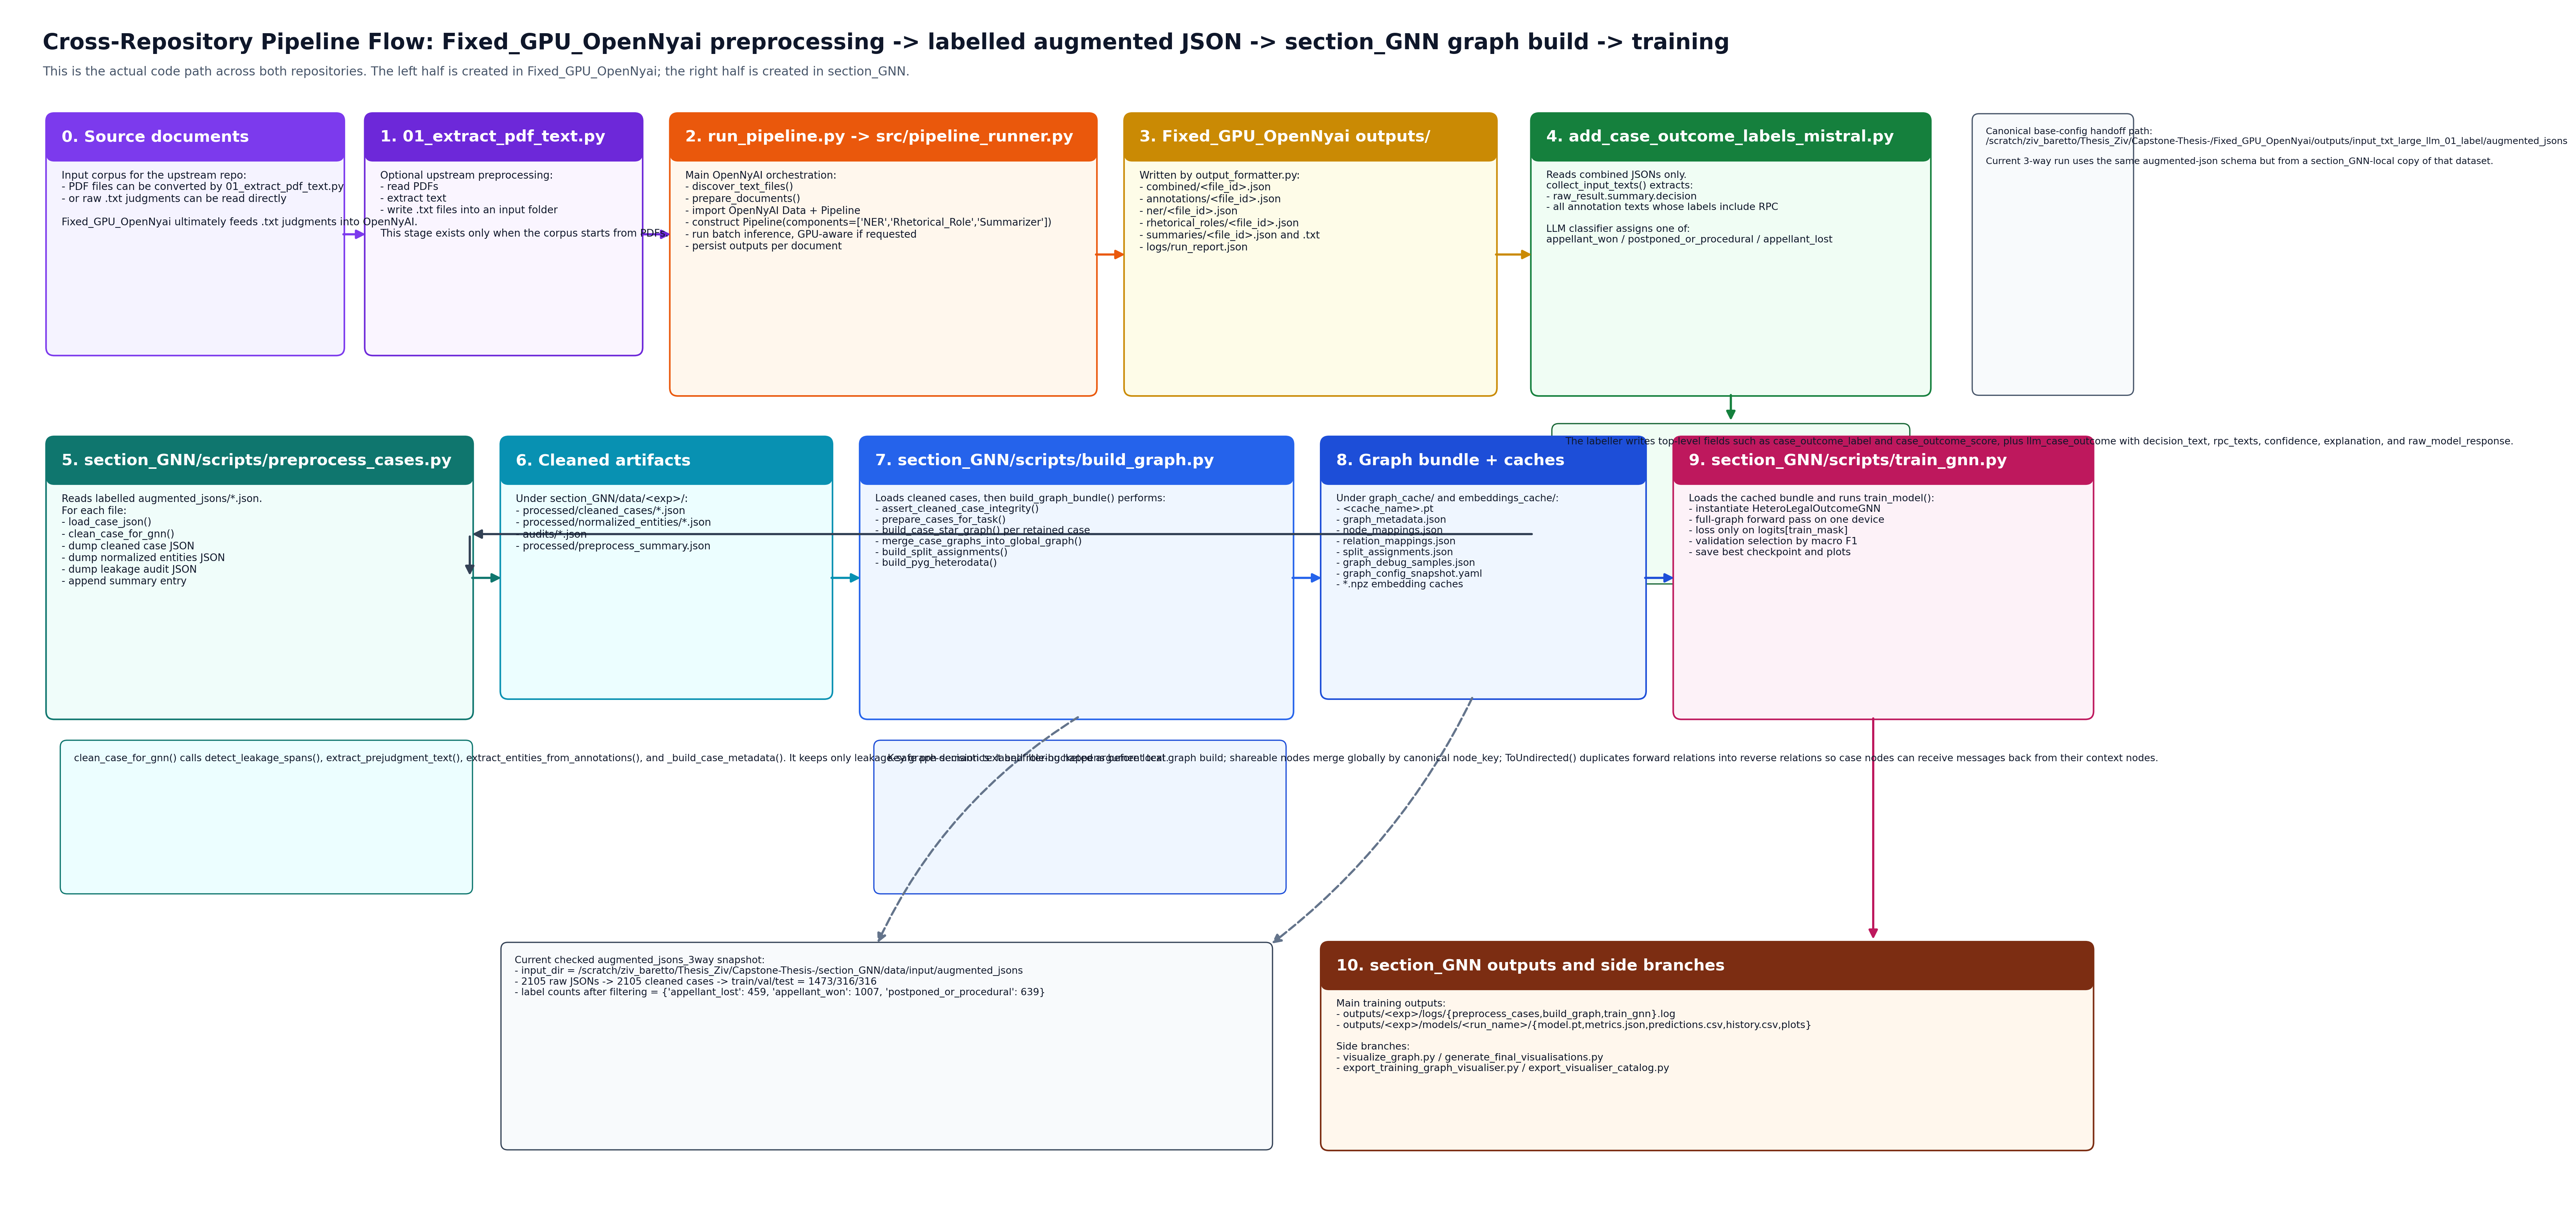
\includegraphics[width=\textwidth,height=0.86\textheight,keepaspectratio]{figures/section_gnn_pipeline_flow.png}
\end{frame}

\section{Input and Intermediate Data}

\begin{frame}{Raw Input Schema}
\small
The implementation expects the upstream JSON to expose these fields when available:

\begin{itemize}
  \item \code{case_outcome_label}
  \item \code{raw_result.summary.PREAMBLE}
  \item \code{raw_result.summary.facts}
  \item \code{raw_result.summary.arguments}
  \item \code{raw_result.summary.decision}
  \item \code{raw_result.data.text}
  \item \code{raw_result.data.preamble_end_char_offset}
  \item \code{raw_result.annotations[*]}
\end{itemize}

Each annotation can provide:

\begin{itemize}
  \item \code{id}, \code{summary_section}, \code{labels}, \code{text}
  \item \code{entities[*].text}
  \item \code{entities[*].normalized_name}
  \item \code{entities[*].labels}
  \item \code{entities[*].start}, \code{entities[*].end}
\end{itemize}
\end{frame}

\begin{frame}{Leakage Handling and CleanedCase}
\small
\begin{block}{Fields explicitly removed or audited}
\code{case_outcome_label}, \code{case_outcome_score}, \code{llm_case_outcome}, \code{decision_text}, \code{rpc_texts}, \code{short_explanation}, \code{raw_model_response}, and \code{raw_result.summary.decision}.
\end{block}

\begin{block}{Retained text fields}
\code{preamble}, \code{facts}, \code{arguments}, \code{petitioner_arguments}, \code{respondent_arguments}, \code{other_lawyer_arguments}.
\end{block}

\begin{block}{CleanedCase fields}
\code{case_id}, \code{file_name}, \code{file_id}, \code{internal_file_id}, \code{source_path}, \code{raw_label}, \code{texts}, \code{metadata}, \code{entities}, \code{leakage_audit}.
\end{block}
\end{frame}

\begin{frame}{Normalization and Heuristics}
\small
\begin{itemize}
  \item Judges and lawyers lose honorifics before punctuation stripping.
  \item Courts get boilerplate normalized.
  \item Statute/provision mentions normalize abbreviations such as \code{sec.}, \code{u/s}, and \code{cr.p.c.}
  \item \code{LAWYER} is retyped to \code{petitioner_lawyer}, \code{defence_lawyer}, or left as \code{lawyer} by scanning nearby text.
  \item Argument annotations can be copied into \code{petitioner_arguments}, \code{respondent_arguments}, or \code{other_lawyer_arguments}.
  \item Petition type is inferred only from preamble text using a small list of markers such as \code{writ petition}, \code{appeal}, and \code{bail application}.
\end{itemize}
\end{frame}

\section{Graph Ontology}

\begin{frame}{Node Types: Text and Root Nodes}
\scriptsize
\begin{tabularx}{\textwidth}{>{\raggedright\arraybackslash}p{0.22\textwidth}p{0.17\textwidth}Y}
\toprule
Node Type & Shared? & Meaning \\
\midrule
\code{case} & no & Root prediction target; text is concatenated base text sections, metadata carries counts/lengths/year/petition type/file info/raw label. \\
\code{preamble} & no & Retained preamble text node. \\
\code{facts} & no & Retained facts text node. \\
\code{arguments} & no & Retained general arguments text node. Main citation hub. \\
\code{petitioner_arguments} & no & Petitioner/appellant-side argument bucket. \\
\code{respondent_arguments} & no & Respondent/state-side argument bucket. \\
\code{other_lawyer_arguments} & no & Lawyer argument bucket with no confident side assignment. \\
\bottomrule
\end{tabularx}
\end{frame}

\begin{frame}{Node Types: Parties, Bench, Counsel, Authorities}
\scriptsize
\begin{tabularx}{\textwidth}{>{\raggedright\arraybackslash}p{0.24\textwidth}p{0.12\textwidth}Y}
\toprule
Node Type & Shared by Default? & Meaning \\
\midrule
\code{petitioner} & no & Party entity. Can be shared only if \code{share_party_nodes} is enabled. \\
\code{respondent} & no & Party entity. Can be shared only if \code{share_party_nodes} is enabled. \\
\code{court} & yes & Normalized court or bench node. \\
\code{judge} & yes & Normalized judge node. \\
\code{petitioner_lawyer} & yes & Lawyer inferred to represent the petitioner/appellant side. \\
\code{defence_lawyer} & yes & Lawyer inferred to represent the respondent/state side. \\
\code{lawyer} & yes & Lawyer not confidently assigned to either side. \\
\code{statute} & yes & Legislation node; can also be created synthetically from a provision linkage. \\
\code{provision} & yes & Section/rule/provision node. \\
\code{precedent} & yes & Prior-case citation. \\
\bottomrule
\end{tabularx}
\end{frame}

\begin{frame}{Node Types: Context Nodes}
\scriptsize
\begin{tabularx}{\textwidth}{>{\raggedright\arraybackslash}p{0.24\textwidth}p{0.12\textwidth}Y}
\toprule
Node Type & Shared by Default? & Meaning \\
\midrule
\code{org} & yes & Organization mention. \\
\code{gpe} & yes & Geopolitical/place mention. \\
\code{date} & yes & Date mention. Also used for heuristic year extraction at preprocessing time. \\
\code{case_number} & yes & Case/FIR/reference number mention. \\
\bottomrule
\end{tabularx}

\vspace{0.3cm}

\begin{block}{Node metadata}
\scriptsize
Case nodes store case-level metadata plus \code{raw_label}. Text nodes store \code{text_length} and argument-link counters. Entity nodes store \code{mention_count}, \code{first_seen_section}, \code{seen_in_arguments}, \code{seen_in_preamble}, \code{linked_statute_canonical}, and \code{is_shared_node}.
\end{block}
\end{frame}

\begin{frame}{Edge Types I: Case to Text and Core Entities}
\scriptsize
\begin{tabularx}{\textwidth}{>{\raggedright\arraybackslash}p{0.28\textwidth}p{0.24\textwidth}Y}
\toprule
Edge Type & Created When & Meaning \\
\midrule
\code{case -has_preamble-> preamble} & preamble text exists & Link case to preamble text. \\
\code{case -has_facts-> facts} & facts text exists & Link case to facts text. \\
\code{case -has_arguments-> arguments} & arguments text exists & Link case to general arguments text. \\
\code{case -has_petitioner_arguments-> petitioner_arguments} & petitioner bucket exists & Link case to petitioner-side argument text. \\
\code{case -has_respondent_arguments-> respondent_arguments} & respondent bucket exists & Link case to respondent-side argument text. \\
\code{case -has_other_lawyer_arguments-> other_lawyer_arguments} & other bucket exists & Link case to unassigned-lawyer argument text. \\
\code{case -has_petitioner-> petitioner} & petitioner entity exists & Link case to petitioner entity. \\
\code{case -has_respondent-> respondent} & respondent entity exists & Link case to respondent entity. \\
\code{case -heard_in-> court} & court entity exists & Link case to court. \\
\code{case -decided_by_bench-> judge} & judge entity exists & Link case to judge. \\
\bottomrule
\end{tabularx}
\end{frame}

\begin{frame}{Edge Types II: Counsel and Context}
\scriptsize
\begin{tabularx}{\textwidth}{>{\raggedright\arraybackslash}p{0.28\textwidth}p{0.24\textwidth}Y}
\toprule
Edge Type & Created When & Meaning \\
\midrule
\code{case -has_lawyer-> lawyer} & generic lawyer exists & Link case to side-unknown lawyer. \\
\code{case -has_petitioner_lawyer-> petitioner_lawyer} & petitioner-side lawyer exists & Link case to petitioner lawyer. \\
\code{case -has_defence_lawyer-> defence_lawyer} & respondent-side lawyer exists & Link case to defence lawyer. \\
\code{case -mentions_org-> org} & organization entity exists & Link case to organization mention. \\
\code{case -mentions_gpe-> gpe} & GPE entity exists & Link case to place mention. \\
\code{case -has_date-> date} & date entity exists & Link case to date mention. \\
\code{case -has_case_number-> case_number} & case-number entity exists & Link case to case-number/reference mention. \\
\bottomrule
\end{tabularx}
\end{frame}

\begin{frame}{Edge Types III: Citations and Bridging Edges}
\tiny
\begin{tabularx}{\textwidth}{>{\raggedright\arraybackslash}p{0.30\textwidth}Y}
\toprule
Edge Type & Meaning \\
\midrule
\code{arguments -cites_statute-> statute} & Statute was seen in arguments text. \\
\code{arguments -cites_provision-> provision} & Provision was seen in arguments text. \\
\code{arguments -cites_precedent-> precedent} & Precedent was seen in arguments text. \\
\code{provision -belongs_to_statute-> statute} & Provision annotation carried an associated statute name. \\
\code{petitioner_lawyer -citation-> arguments} & Petitioner lawyer connected to general arguments node. \\
\code{defence_lawyer -citation-> arguments} & Defence lawyer connected to general arguments node. \\
\code{petitioner_lawyer -citation-> petitioner_arguments} & Petitioner lawyer connected to petitioner-only argument bucket. \\
\code{defence_lawyer -citation-> respondent_arguments} & Defence lawyer connected to respondent-only argument bucket. \\
\code{lawyer -citation-> other_lawyer_arguments} & Generic lawyer connected to other-lawyer argument bucket. \\
\code{provision -used_in_arguments-> arguments} & Shortens path from provision to arguments. \\
\code{statute -used_in_arguments-> arguments} & Shortens path from statute to arguments. \\
\code{petitioner -is_party_in_arguments-> arguments} & Petitioner bridged into generic arguments. \\
\code{respondent -is_party_in_arguments-> arguments} & Respondent bridged into generic arguments. \\
\code{petitioner -is_party_in_arguments-> petitioner_arguments} & Petitioner bridged into petitioner-specific arguments. \\
\code{respondent -is_party_in_arguments-> respondent_arguments} & Respondent bridged into respondent-specific arguments. \\
\code{judge -presided_arguments-> arguments} & Judge bridged into arguments. \\
\bottomrule
\end{tabularx}
\end{frame}

\begin{frame}{Reverse Edges and Graph Merge}
\small
\begin{block}{Reverse edges}
\code{build_pyg_heterodata()} applies \code{ToUndirected} when \code{graph.use_to_undirected} is true. Every forward relation becomes a reverse relation named \code{rev_<relation>}. Current graph caches contain 33 forward + 33 reverse = 66 relation types.
\end{block}

\begin{block}{Global merge behavior}
\begin{itemize}
  \item Shared nodes are deduplicated by \code{node_key}.
  \item Edges are deduplicated by source key, relation, and target key.
  \item Metadata adds \code{global_case_frequency} and \code{degree}.
  \item Current shared types include court, judge, lawyers, statutes, provisions, precedents, org, gpe, date, and case number.
\end{itemize}
\end{block}
\end{frame}

\section{Features}

\begin{frame}{Feature Construction}
\small
\begin{tabularx}{\textwidth}{>{\raggedright\arraybackslash}p{0.20\textwidth}Y}
\toprule
Node Family & Implemented Feature Vector \\
\midrule
\code{case} & text embedding of concatenated configured base text sections + 12 case scalar slots. \\
\code{text nodes} & text embedding of the section text + 12 text scalar slots. \\
\code{entity nodes} & text embedding of the normalized entity string + 12 scalar slots, of which the first 10 are used by entity features in current configs. \\
\bottomrule
\end{tabularx}

\vspace{0.3cm}

\begin{block}{Current experiment dimensions}
\begin{itemize}
  \item \code{food_law_final}: 384 embedding + 12 scalar = 396
  \item \code{augmented_jsons_3way}: 768 embedding + 12 scalar = 780
\end{itemize}
\end{block}
\end{frame}

\begin{frame}{Text Encoders and Cache}
\small
\begin{itemize}
  \item \code{sentence_transformers}: used in the binary food-law run with \code{all-MiniLM-L6-v2}.
  \item \code{hf_encoder}: used in the 3-way run with \code{saibo/legal-roberta-base}.
  \item \code{hashing}: deterministic fallback and sanity backend.
\end{itemize}

\begin{block}{Cache behavior}
\begin{itemize}
  \item embeddings are cached as \code{.npz} files under \code{embeddings_cache_dir},
  \item cache key uses backend/model config, node ids, and text lengths,
  \item the cache key does not hash the full text content itself.
\end{itemize}
\end{block}
\end{frame}

\section{Model}

\begin{frame}{HeteroLegalOutcomeGNN Architecture}
\small
\begin{itemize}
  \item one input projection \code{Linear(input_dim, hidden_dim)} per node type
  \item one learned type embedding per node type
  \item one \code{LayerNorm(hidden_dim)} per node type per layer
  \item repeated message-passing layers:
  \begin{itemize}
    \item \code{HGTConv} if \code{architecture = hgt}
    \item \code{HeteroConv} with per-edge-type \code{SAGEConv} if \code{architecture = heteroconv} or \code{rgcn}
  \end{itemize}
  \item final \code{MLPHead} = \code{Linear -> ReLU -> Dropout -> Linear}
\end{itemize}

\begin{block}{What does not exist}
No edge features, no pooling layer, no jump knowledge, no true separate RGCN implementation, no batching logic.
\end{block}
\end{frame}

\begin{frame}{Detailed GNN Architecture Figure}
  \centering
  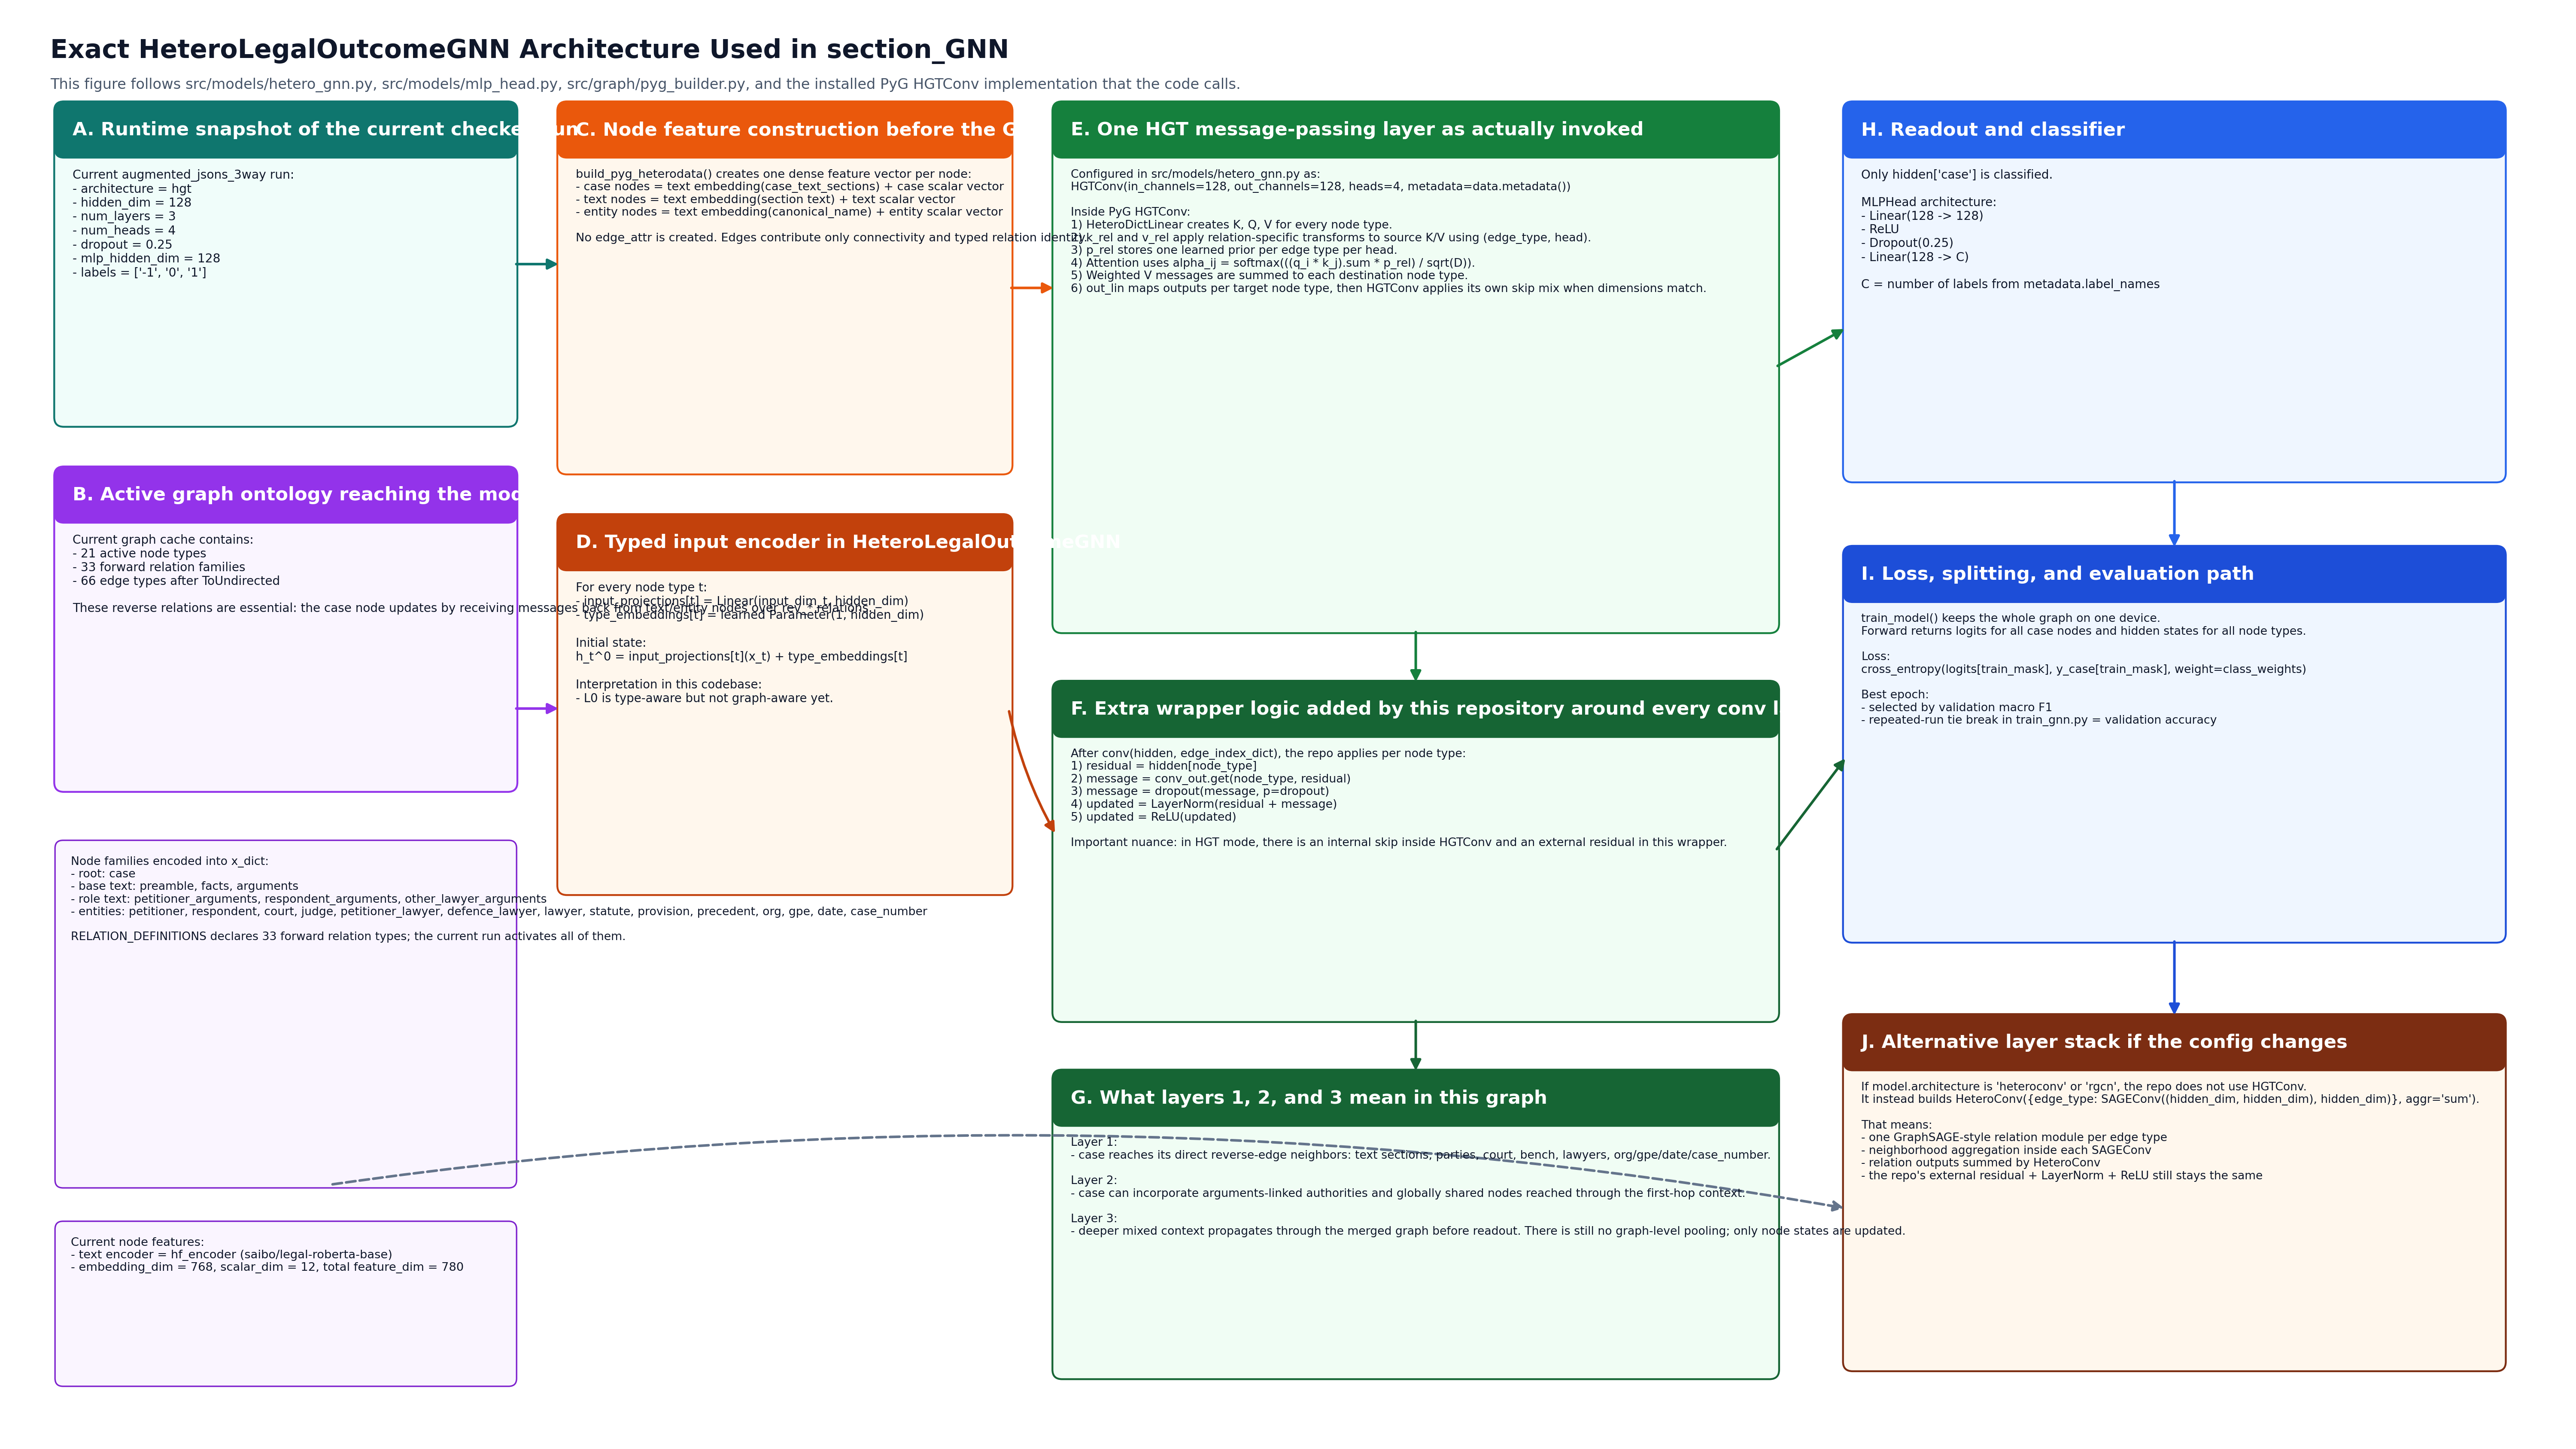
\includegraphics[width=\textwidth,height=0.86\textheight,keepaspectratio]{figures/section_gnn_gnn_architecture.png}
\end{frame}

\begin{frame}{Exact \code{forward()} Flow}
\small
\begin{enumerate}
  \item Project every node type into \code{hidden_dim} and add its type embedding.
  \item For each message-passing layer:
  \begin{enumerate}
    \item cache the current hidden dict as \code{residual},
    \item compute \code{conv_out = conv(hidden, edge_index_dict)},
    \item for each node type:
    \begin{enumerate}
      \item use the convolution output if present, otherwise keep the residual tensor,
      \item apply dropout,
      \item add the residual tensor,
      \item apply the node-type-specific layer norm,
      \item apply \code{ReLU}.
    \end{enumerate}
  \end{enumerate}
  \item Apply the MLP head only to \code{hidden["case"]}.
  \item Return:
  \begin{itemize}
    \item case logits
    \item the final hidden-state dictionary for all node types
  \end{itemize}
\end{enumerate}
\end{frame}

\section{Labels, Splits, and Training}

\begin{frame}{Label Mapping and Split Logic}
\small
\begin{block}{Task modes}
\code{binary} and \code{multiclass}. The 3-way setup is just \code{multiclass}.
\end{block}

\begin{block}{Binary mapping}
\code{appellant_won -> win}, \code{appellant_lost -> lose}, \code{postponed_or_procedural -> null} with dropping enabled.
\end{block}

\begin{block}{3-way mapping}
\code{appellant_lost -> -1}, \code{postponed_or_procedural -> 0}, \code{appellant_won -> 1}.
\end{block}

\begin{block}{Split modes}
\code{random}, \code{year}, and \code{court}. Random mode tries stratification and falls back to unstratified splits if necessary. Grouped modes preserve groups but do not stratify.
\end{block}
\end{frame}

\begin{frame}{Training Loop and Selection Rule}
\small
\begin{itemize}
  \item full graph is moved to one device
  \item optimizer: \code{AdamW}
  \item loss: cross entropy over \code{logits[train_mask]}
  \item optional balanced class weights from scikit-learn
  \item best epoch inside a run is chosen by validation macro F1
  \item optional early stopping on patience over validation macro F1
  \item final train/val/test metrics are computed on the best checkpoint
\end{itemize}

\begin{block}{Repeated runs}
If \code{repeat_runs > 1}, seeds advance by \code{seed_stride}; each run writes its own directory; best run is selected by validation macro F1 with validation accuracy as tie-breaker.
\end{block}
\end{frame}

\begin{frame}{Metrics and Training Artifacts}
\small
\begin{tabularx}{\textwidth}{>{\raggedright\arraybackslash}p{0.28\textwidth}Y}
\toprule
Artifact & Meaning \\
\midrule
\code{model.pt} & Best state dict only. \\
\code{metrics.json} & Train/val/test metrics, best epoch, best validation macro F1, epoch history. \\
\code{predictions.csv} & Per-case predictions with raw labels, mapped labels, split, and confidence. \\
\code{history.csv} & Flat table version of the epoch history. \\
\code{training_history.png} & Train loss and macro-F1 curves. \\
\code{split_metrics.png} & Accuracy, macro F1, micro F1 per split. \\
\code{confusion_matrix_*.png} & Confusion matrix per split. \\
\code{multi_run_summary.json} & Repeated-run summary and best-run selection record. \\
\bottomrule
\end{tabularx}
\end{frame}

\section{Configs and Current Results}

\begin{frame}{Config Variants}
\scriptsize
\begin{tabularx}{\textwidth}{>{\raggedright\arraybackslash}p{0.34\textwidth}Y}
\toprule
Config & Key Differences \\
\midrule
\code{gnn_case_star.yaml} & Base binary config, MiniLM embeddings, no role-argument nodes in the graph, older \code{GNN/} path layout. \\
\code{gnn_case_star_food_law_final.yaml} & Binary food-law run, role-argument nodes enabled, MiniLM embeddings, repeated runs, no early stopping. \\
\code{gnn_case_star_augmented_jsons_3way.yaml} & 3-way run, role-argument nodes enabled, Hugging Face legal-RoBERTa encoder, labels \code{-1}/\code{0}/\code{1}. \\
\code{gnn_case_star_sanity.yaml} & Hashing encoder, smaller model, fewer epochs, fast sanity path. \\
\bottomrule
\end{tabularx}

\vspace{0.25cm}

Common ablation variants: \code{text_only}, \code{star_only}, \code{without_judge}, \code{without_statute_provision}, \code{without_preamble}, \code{facts_only}, \code{arguments_only}.
\end{frame}

\begin{frame}{Current Binary Food-Law Artifact Snapshot}
\small
\begin{itemize}
  \item retained cases: 1466
  \item dropped procedural cases: 639
  \item feature dim: 396
  \item split sizes: 1026 / 220 / 220
  \item repeated runs: 3
  \item selected run: \code{run_03_seed_44}
\end{itemize}

\begin{center}
\begin{tabular}{lrr}
\toprule
Split & Accuracy & Macro F1 \\
\midrule
Train & 0.9951 & 0.9944 \\
Val & 0.8591 & 0.8300 \\
Test & 0.7636 & 0.7108 \\
\bottomrule
\end{tabular}
\end{center}
\end{frame}

\begin{frame}{Current 3-Way Artifact Snapshot}
\small
\begin{itemize}
  \item retained cases: 2105
  \item dropped cases: 0
  \item label distribution:
  \begin{itemize}
    \item \code{appellant_lost}: 459
    \item \code{postponed_or_procedural}: 639
    \item \code{appellant_won}: 1007
  \end{itemize}
  \item feature dim: 780
  \item split sizes: 1473 / 316 / 316
\end{itemize}

\begin{center}
\begin{tabular}{lrr}
\toprule
Split & Accuracy & Macro F1 \\
\midrule
Train & 0.9722 & 0.9715 \\
Val & 0.7215 & 0.6961 \\
Test & 0.7215 & 0.6937 \\
\bottomrule
\end{tabular}
\end{center}
\end{frame}

\section{Visualization}

\begin{frame}{Visualization Subsystems}
\small
\begin{block}{Static figure pipeline}
\code{src/visualization/graph_visualizer.py} and \code{src/visualization/final_visualizer.py} generate explanatory PNGs for schema, local graphs, receptive fields, and training explanations.
\end{block}

\begin{block}{Browser visualizer}
\begin{itemize}
  \item \code{visualiser/index.html}: D3 graph view
  \item \code{visualiser/stats/index.html}: stats dashboard
  \item \code{visualiser/layers/index.html}: graph/model layer explainer
  \item exact graph export: \code{scripts/export_training_graph_visualiser.py}
  \item sampled fallback export: \code{scripts/export_visualiser_catalog.py}
\end{itemize}
\end{block}
\end{frame}

\section{Limitations and Extension Points}

\begin{frame}{Code-Grounded Limitations}
\small
\begin{itemize}
  \item Leakage detection is phrase-based, not semantic.
  \item Lawyer-side inference is heuristic and window-based.
  \item Party normalization is weak in current artifacts; party node counts are extremely large relative to case count.
  \item The graph is transductive: train/val/test share authority nodes.
  \item There are no edge features or edge weights.
  \item Training is full-graph only; there is no minibatching or neighbor sampling.
  \item The embedding cache key does not hash full text content.
\end{itemize}
\end{frame}

\begin{frame}{Ambiguities and Extension Points}
\small
\begin{block}{Current ambiguities}
\begin{itemize}
  \item \code{include_reverse_edges} exists in YAML but runtime behavior is actually driven by \code{use_to_undirected}.
  \item \code{allowed_summary_fields} exists in YAML but extraction currently reads a fixed section map.
  \item \code{RELATION_DEFINITIONS} is descriptive; changing it alone does not change runtime graph construction.
  \item \code{rgcn} is only an alias for the \code{HeteroConv + SAGEConv} path.
\end{itemize}
\end{block}

\begin{block}{High-value extension points}
\begin{itemize}
  \item stronger leakage detection
  \item better party normalization
  \item content-safe embedding cache keys
  \item edge attributes or weights
  \item new hetero backbones beyond HGT and HeteroConv/SAGEConv
  \item mini-batch or sampled training
  \item executable centralized graph schema
\end{itemize}
\end{block}
\end{frame}

\begin{frame}{Bottom Line}
\small
\repo{} is a complete leakage-aware heterogeneous legal GNN pipeline with:

\begin{itemize}
  \item a real preprocessing contract,
  \item a non-trivial graph ontology including role-specific argument nodes and bridging edges,
  \item a simple but inspectable hetero GNN implementation,
  \item reproducible graph caches and run artifacts,
  \item both static and browser-based graph inspection tooling.
\end{itemize}

Its most important implementation caveats are the heuristic preprocessing rules, transductive global graph, sparse/noisy party normalization, and a few configuration keys that are descriptive rather than authoritative.
\end{frame}

\end{document}
